
 \chapter{Hasil Uji Coba Kebenaran pada Situs SPOJ}
  %\setcounter{figure}{0}
   
   \begin{figure}[H]
   \centering
  	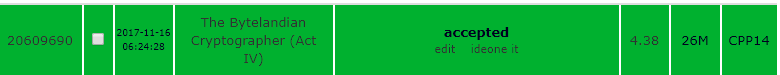
\includegraphics[scale=0.53]{images/lampiran/best.png}
  	\caption{Hasil Uji Coba pada Situs Penilaian SPOJ}
  	\label{fig:best_submission}
  	\end{figure}
	
	 \begin{figure}[H]
  \centering
  	 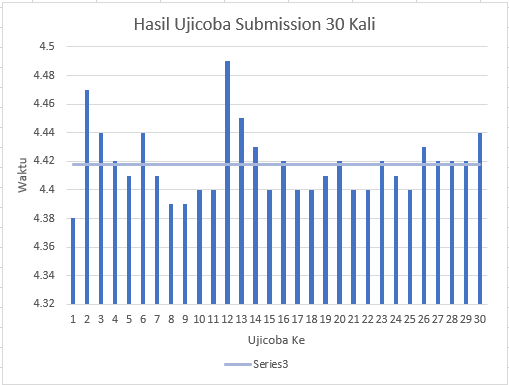
\includegraphics[scale=0.7]{images/lampiran/uji31.png}
  	\caption{Grafik Hasil Uji Coba pada Situs SPOJ Sebanyak 30 Kali}
  	\label{fig:chart}
  \end{figure}  	
  	
  	\begin{figure}[H]
  	\centering
  	 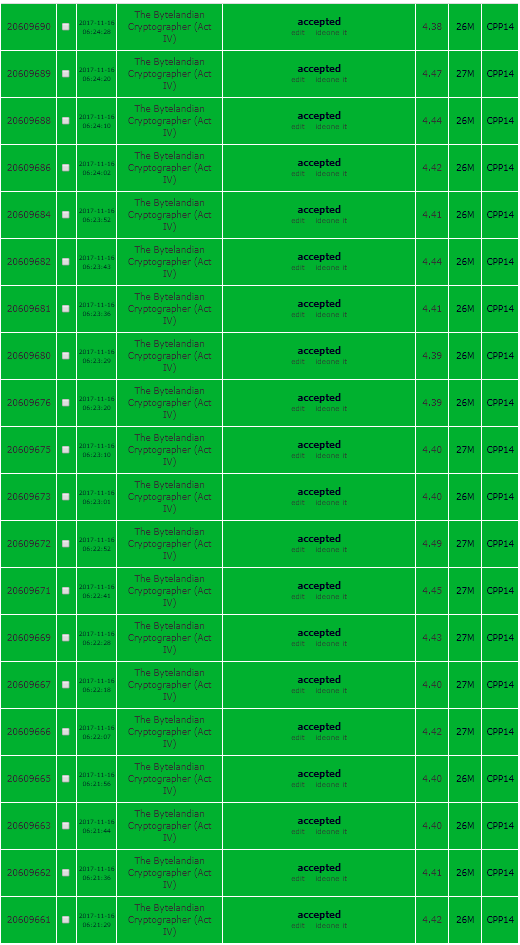
\includegraphics[scale=0.63]{images/lampiran/uji1.png}
  	\caption{Hasil Pengujian Sebanyak 30 Kali pada Situs Penilaian Daring SPOJ (1)}
  	\label{fig:submission1}
  \end{figure}
  
  \begin{figure}[H]
  \centering
  	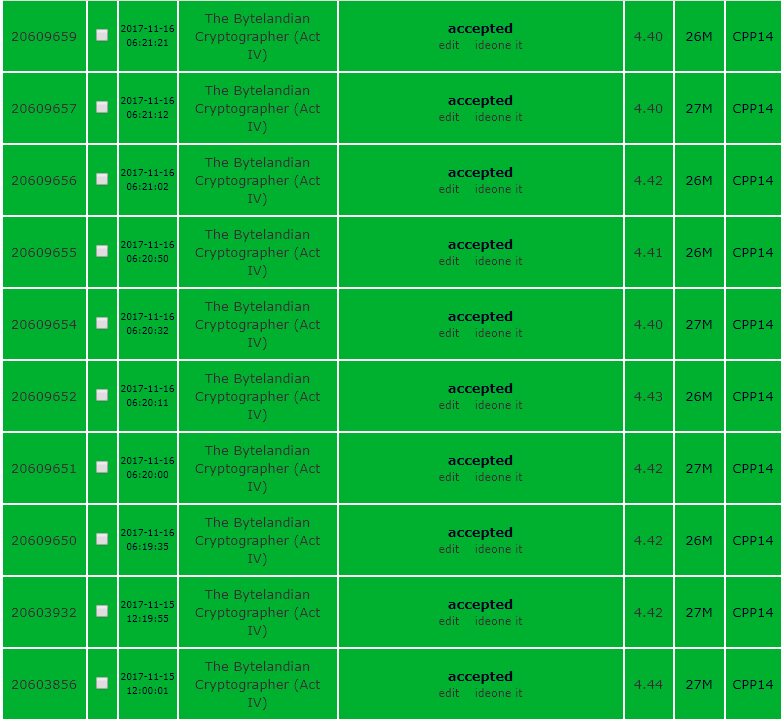
\includegraphics[scale=0.5]{images/lampiran/uji3.png}
  	\caption{Hasil Pengujian Sebanyak 30 Kali pada Situs Penilaian Daring SPOJ (2)}
  	\label{fig:submission2}
  \end{figure}
  
  \begin{figure}[H]
  \centering
  	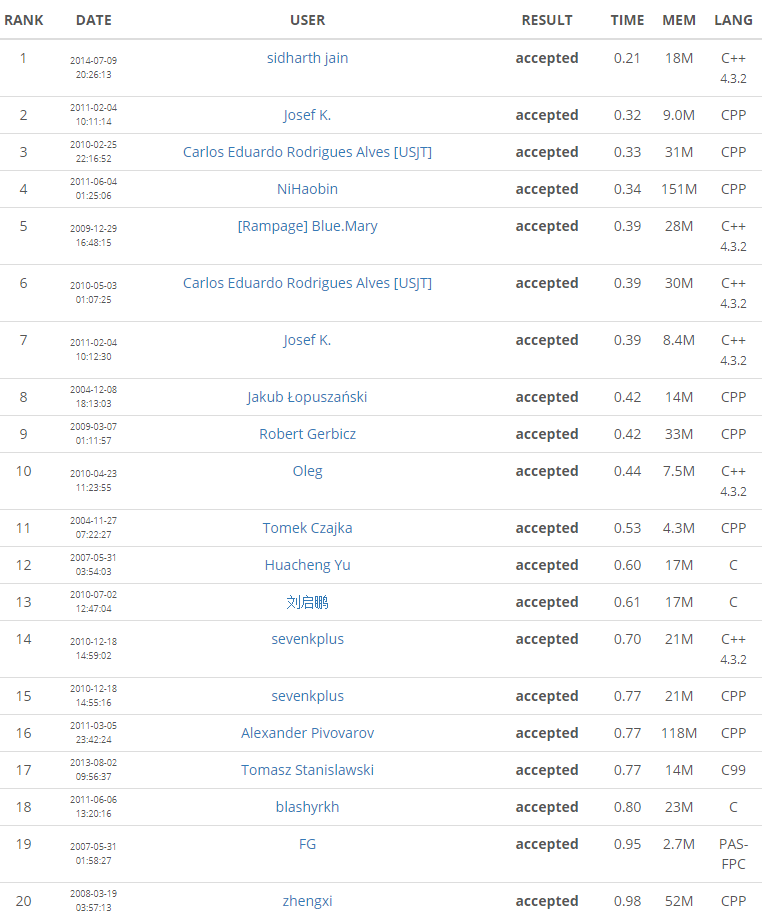
\includegraphics[scale=0.55]{images/lampiran/rankdiatas1.png}
  	\caption{Peringkat yang lebih tinggi dari program ini (1)}
  	\label{fig:submission2}
  \end{figure}
  
  \begin{figure}[H]
  \centering
  	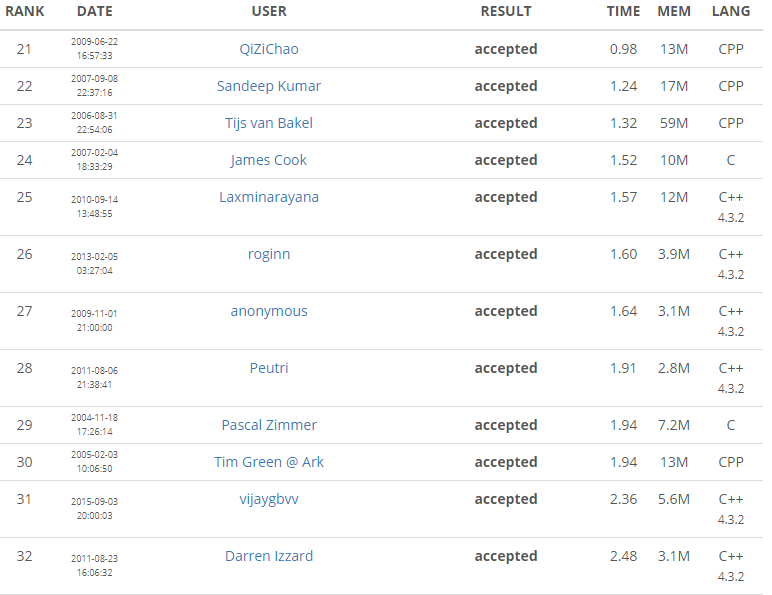
\includegraphics[scale=0.55]{images/lampiran/rankdiatas2.png}
  	\caption{Peringkat yang lebih tinggi dari program ini (2)}
  	\label{fig:submission2}
  \end{figure}
  
  
  
 
  
  
